% !TEX root = ../thesis.tex

\chapter{Nasadenie}\label{ch:deployment}

\section{Kontajnery}

Celý systém je zabalený do kontajnerov. Na lokálny vývoj a demonštráciu sa spúšťa pomocou Docker Compose. Základ tvoria štyri kontajnery (tabuľka~\ref{tab:containers}).

\begin{table}[ht]
  \centering
  \caption{Kontajnery systému}\label{tab:containers}
  \begin{tabular}{@{}llp{.5\textwidth}@{}}
    \toprule
    Kontajner & Port & Obsah \\
    \midrule
    \texttt{db-main} & 5432 & PostgreSQL 17, databáza \texttt{salon\_main} \\
    \texttt{db-ml}   & 5433 & PostgreSQL 17, databáza \texttt{salon\_ml} \\
    \texttt{app}     & 8080 & ASP.NET Core API spolu so zostaveným frontendom \\
    \texttt{ml}      & 8000 & FastAPI a ML pipeline \\
    \bottomrule
  \end{tabular}
\end{table}

Obraz \texttt{app} sa zostavuje viacstupňovo: najprv sa v Node.js zostaví frontend, potom sa v .NET SDK skompiluje backend a nakoniec sa oba výstupy skopírujú do runtime obrazu ASP.NET Core. Hlavný backend tak servíruje statické súbory frontendu a všetky cesty mimo \texttt{/api} presmeruje na \texttt{index.html}, kým neznáma API cesta vráti chybu 404 vo formáte JSON. Pri štarte kontajnera sa automaticky aplikujú databázové migrácie a naplnia sa ukážkové dáta. Kontajner \texttt{ml} pri štarte aplikuje migrácie nástrojom Alembic a spustí server uvicorn.

Databázy majú zdravotné kontroly (\texttt{pg\_isready}) a backendy štartujú až po tom, čo je ich databáza pripravená. Dáta oboch databáz a natrénované modely sú uložené v pomenovaných zväzkoch, takže prežijú reštart aj výmenu kontajnerov. Konfigurácia a tajomstvá (heslá databáz, interný API kľúč, povolené originy pre CORS, adresa ML služby) sa odovzdávajú výhradne cez premenné prostredia zo súboru \texttt{.env}.

Lokálne sa celý systém spustí príkazom \texttt{docker compose up -{}-build} a je dostupný na adrese \url{http://localhost:8080}.

\section{Nasadenie na Azure}

V produkcii sa namiesto Docker Compose použijú spravované služby platformy Microsoft Azure (obrázok~\ref{fig:deployment}). Oba backendy bežia ako kontajnery v službe Azure App Service (Web App for Containers) a databázy poskytuje služba Azure Database for PostgreSQL. Azure sa tak stará o prevádzku servera, aktualizácie, HTTPS certifikáty aj zálohovanie databáz.

\begin{figure}[ht]
  \centering
  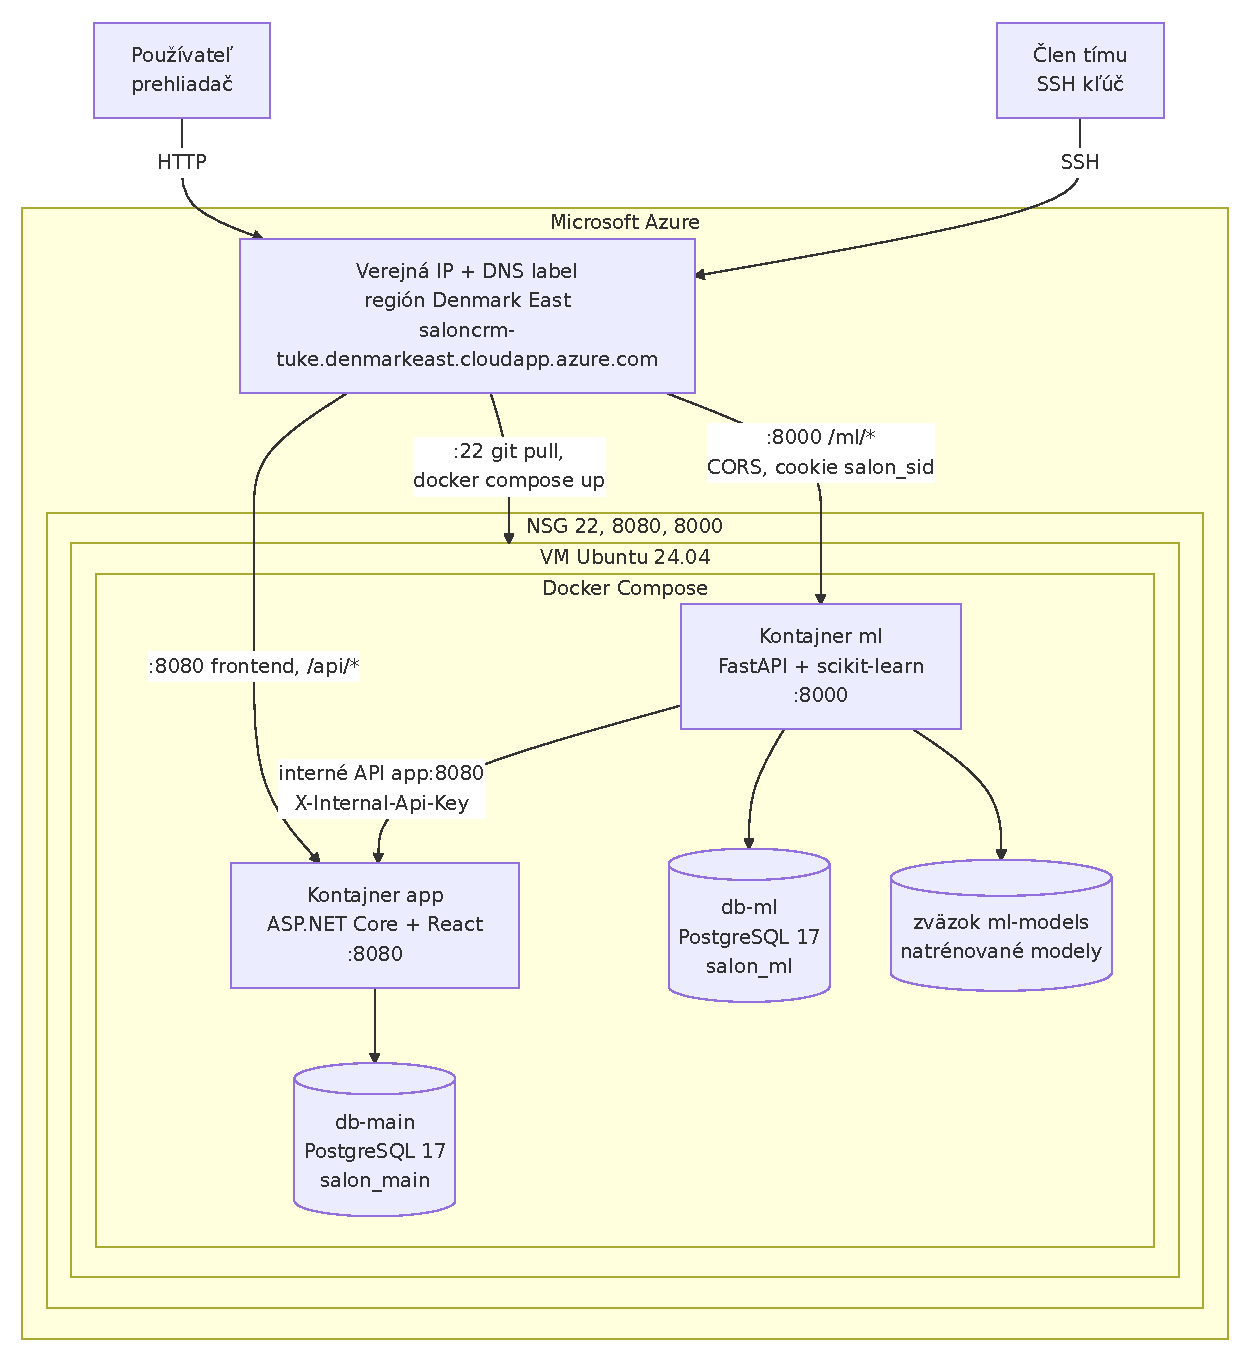
\includegraphics[width=\textwidth]{figures/deployment.pdf}
  \caption{Nasadenie v Azure}\label{fig:deployment}
\end{figure}

\subsection*{Aplikácie}

V jednom App Service pláne s Linuxom bežia dve webové aplikácie. Každá spúšťa ten istý Docker obraz, ktorý sa používa lokálne:

\begin{description}
  \item[Web App \texttt{app}] hlavný backend spolu so zostaveným frontendom,
  \item[Web App \texttt{ml}] ML backend.
\end{description}

App Service zabezpečuje HTTPS, preto sa cookie \texttt{salon\_sid} posiela s príznakom \texttt{Secure}. Obe aplikácie dostanú vlastnú doménu ako subdomény jednej registrovanej domény (napr. \nolinkurl{salon.<doména>} a \nolinkurl{ml.<doména>}). Predvolené adresy \nolinkurl{*.azurewebsites.net} sa nepoužívajú, pretože prehliadač ich považuje za rôzne weby (\emph{sites}). Cookie so \texttt{SameSite=Lax} by sa potom na ML backend neposlala. Pod spoločnou doménou sa cookie posiela obom backendom rovnako ako pri lokálnom vývoji.

ML backend volá interné API hlavného backendu cez jeho HTTPS adresu, chránené kľúčom v hlavičke \texttt{X-Internal-Api-Key}. Natrénované modely sa ukladajú do trvalého úložiska App Service (adresár \texttt{/home}, premenná \texttt{MODEL\_DIR}), takže prežijú reštart aj nasadenie novej verzie.

\subsection*{Databázy}

Kontajnery \texttt{db-main} a \texttt{db-ml} v produkcii nahrádza Azure Database for PostgreSQL -- Flexible Server s verziou PostgreSQL 17. Na serveri sú dve samostatné databázy, \texttt{salon\_main} a \texttt{salon\_ml}. Každý backend má vlastného databázového používateľa s právami iba na svoju databázu, takže oddelenie dát zostáva zachované. Spojenie je šifrované (TLS) a firewall servera povoľuje prístup iba zo služieb Azure. Rozšírenie \texttt{btree\_gist}, ktoré potrebuje obmedzenie proti prekrývaniu termínov, treba na serveri povoliť v parametri \texttt{azure.extensions}.

\subsection*{Konfigurácia a postup nasadenia}

Konfigurácia sa nastavuje v \emph{Application settings} webových aplikácií. Tie App Service odovzdá kontajneru ako premenné prostredia, rovnako ako súbor \texttt{.env} lokálne. Ide najmä o reťazce pripojenia k databázam, interný API kľúč, adresu hlavného backendu pre ML službu, povolené originy CORS a príznak \texttt{Secure} pre cookie. Adresa ML služby sa zapisuje do frontendu pri zostavení obrazu, preto sa obraz \texttt{app} zostavuje už s produkčnou adresou.

Postup nasadenia:

\begin{enumerate}
  \item vytvorenie skupiny prostriedkov, PostgreSQL servera s dvoma databázami a dvoma používateľmi a povolenie rozšírenia \texttt{btree\_gist},
  \item vytvorenie App Service plánu a dvoch webových aplikácií pre kontajnery,
  \item nastavenie vlastnej domény a certifikátov pre obe aplikácie,
  \item nastavenie \emph{Application settings} (tajomstvá iba tu, nie v repozitári),
  \item zostavenie Docker obrazov v GitHub Actions a ich nahratie do registra kontajnerov,
  \item nasadenie obrazov do webových aplikácií; migrácie databáz sa aplikujú automaticky pri štarte kontajnerov.
\end{enumerate}

Kontinuálna integrácia (GitHub Actions) pri každej zmene zostaví a otestuje všetky časti systému. Rovnaký workflow sa dá rozšíriť o automatické nasadenie nových obrazov po úspešných testoch.
